%%%%%%%%%%%%%%%%%%%%%%%%%%%%%%%%%%%%%%%%%%%%%%%%%%%%%%%%%%%%%%%
%
% Welcome to Overleaf --- just edit your LaTeX on the left,
% and we'll compile it for you on the right. If you open the
% 'Share' menu, you can invite other users to edit at the same
% time. See www.overleaf.com/learn for more info. Enjoy!
%
%%%%%%%%%%%%%%%%%%%%%%%%%%%%%%%%%%%%%%%%%%%%%%%%%%%%%%%%%%%%%%%
% How to Draw Flowcharts in LaTeX using TikZ?
% latexdraw.com
% 30/01/2021 at 00:07

\documentclass[border=0.2cm]{standalone}

% Required packages
\usepackage{tikz}
\usetikzlibrary{shapes,positioning}
\usepackage{makecell}
\usepackage{pgfplots}
\tikzstyle{arrow}=[draw]
\tikzstyle{arrow}=[draw, -latex]

\begin{document}

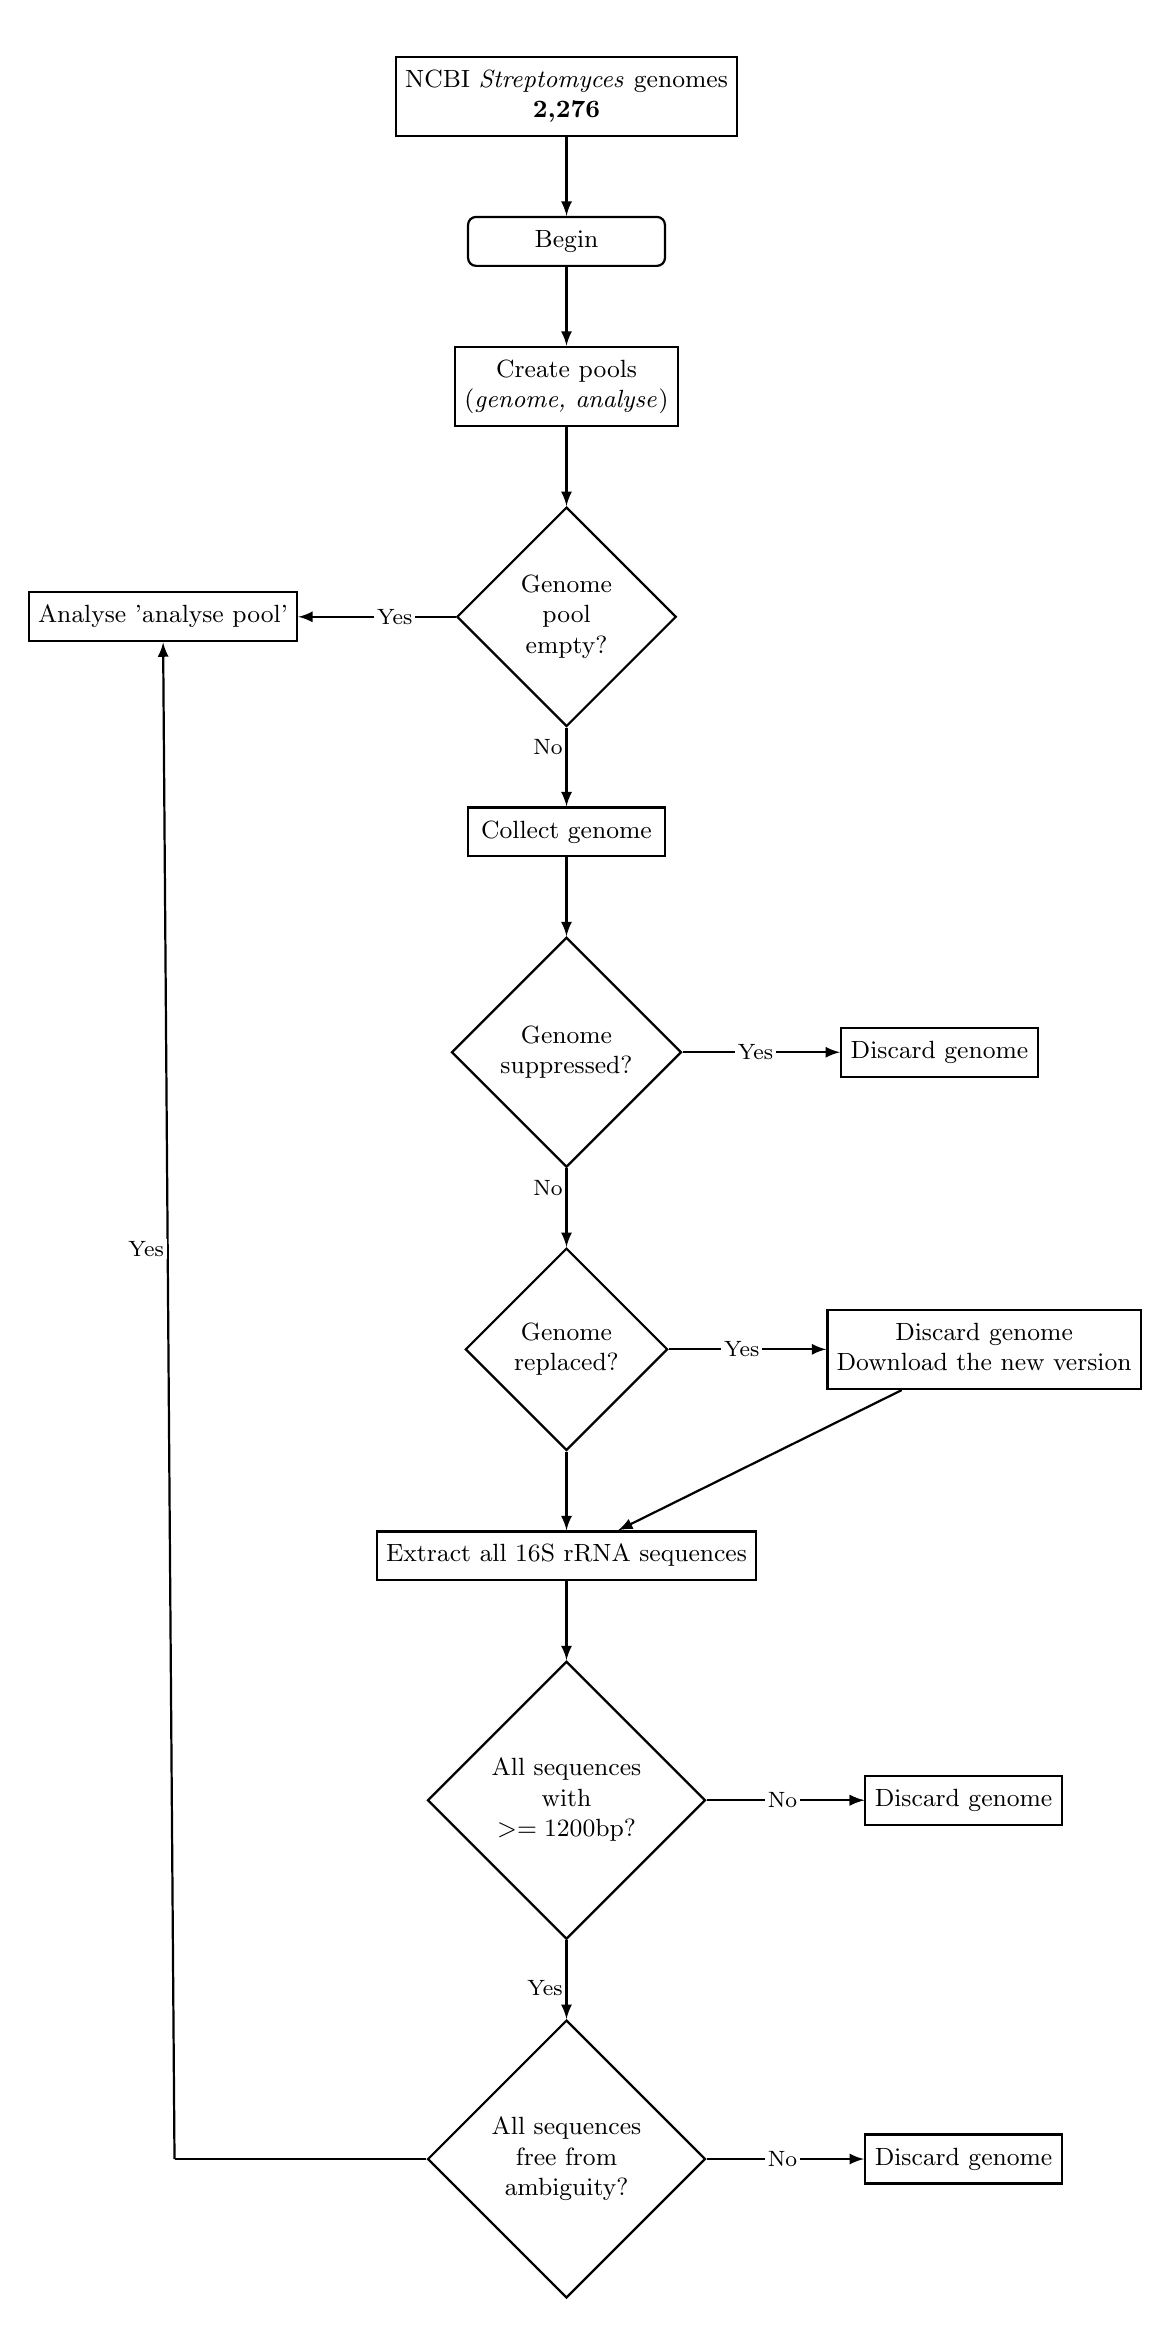
\begin{tikzpicture}[font=\small,thick]



% Conditions test
\node[
    left = 3cm,
    minimum width=1cm] (block1){};

\node[draw,
    below left=0.15cm of block1,
    minimum width=2.5cm] (block2){\makecell[ct]{NCBI \textit{Streptomyces} genomes \\  \textbf{2,276}}};

\node[draw,
    below= 1cm of block2,
    rounded corners=0.1cm,
    minimum width=2.5cm] (block3){\makecell[ct] Begin};


\node[draw,
    below= 1cm of block3,
    minimum width=2.5cm] (block4){\makecell[ct]{Create pools \\ $($\textit{genome, analyse}$)$}};

\node[draw,
    diamond,
    below= 1cm of block4,
    minimum width=2.5cm] (block5){\makecell[ct]{Genome \\pool \\empty$?$ }};

\node[draw,
    left= 2cm of block5,
    minimum width=2.5cm] (block6){\makecell[ct]{Analyse 'analyse pool'}};

\node[draw,
    below= 1cm of block5,
    minimum width=2.5cm] (block7){\makecell[ct]{Collect genome}};

\node[draw,
    diamond,
    below= 1cm of block7,
    minimum width=2.5cm] (block8){\makecell[ct]{Genome \\suppressed$?$ }};

\node[draw,
    right= 2cm of block8,
    minimum width=2.5cm] (block9){\makecell[ct]{Discard genome}};

\node[draw,
    diamond,
    below= 1cm of block8,
    minimum width=2.5cm] (block10){\makecell[ct]{Genome \\replaced$?$ }};

\node[draw,
    right= 2cm of block10,
    minimum width=2.5cm] (block11){\makecell[ct]{Discard genome\\ Download the new version }};

\node[draw,
    below= 1cm of block10,
    minimum width=2.5cm] (block12){\makecell[ct]{Extract all 16S rRNA sequences}};

\node[draw,
    diamond,
    below= 1cm of block12,
    minimum width=2.5cm] (block13){\makecell[ct]{All sequences \\ with\\ $>=1200$bp$?$ }};

\node[draw,
    right= 2cm of block13,
    minimum width=2.5cm] (block14){\makecell[ct]{Discard genome}};

\node[draw,
    diamond,
    below= 1cm of block13,
    minimum width=2.5cm] (block15){\makecell[ct]{All sequences \\ free from \\ambiguity$?$ }};


\node[draw,
    right= 2cm of block15,
    minimum width=2.5cm] (block16){\makecell[ct]{Discard genome}};    

\node[coordinate,left=3.2cm of block15] (block17) {Block 3};


% Arrows
\draw[-latex] (block2) -- (block3);
\draw[-latex] (block3) -- (block4);
\draw[-latex] (block4) -- (block5);
\draw[-latex] (block5) -- (block6) node[pos=0.25,anchor=0,inner sep=1, fill=white]{\footnotesize Yes};
\draw[-latex] (block5) -- (block7) node[pos=0.25,anchor=0,inner sep=1, fill=white]{\footnotesize No};
\draw[-latex] (block7) -- (block8);
\draw[-latex] (block8) -- (block9) node[pos=0.6,anchor=0,inner sep=1, fill=white]{\footnotesize Yes};
\draw[-latex] (block8) -- (block10) node[pos=0.25,anchor=0,inner sep=1, fill=white]{\footnotesize No};
\draw[-latex] (block10) -- (block11) node[pos=0.6,anchor=0,inner sep=1, fill=white]{\footnotesize Yes};
\draw[-latex] (block10) -- (block12);
\draw[-latex] (block12) -- (block13);
\draw[-latex] (block11) -- (block12);
\draw[-latex] (block13) -- (block14) node[pos=0.6,anchor=0,inner sep=1, fill=white]{\footnotesize No};
\draw[-latex] (block13) -- (block15) node[pos=0.6,anchor=0,inner sep=1, fill=white]{\footnotesize Yes};
\draw[-latex] (block13) -- (block14) node[pos=0.6,anchor=0,inner sep=1, fill=white]{\footnotesize No};
\draw[-latex] (block15) -- (block16) node[pos=0.6,anchor=0,inner sep=1, fill=white]{\footnotesize No};
\draw[-latex] (block17) -- (block6) node[pos=0.6,anchor=0,inner sep=1, fill=white]{\footnotesize Yes};

\draw (block15) -| (block17);
\end{tikzpicture}

\end{document}